% Flowchart of the DT-GSK algorithm, in the same clean vertical style as the
% original GSK paper (Fig. 10): rounded terminals, plain (unfilled) process
% boxes, a diamond decision, a loop-back.  No background colours.  Boxes drawn
% with a light SHADED fill are the mechanisms DT-GSK adds to the GSK skeleton.
% Step order matches Algorithm 1 and the frozen code:  ... accept -> ISM
% update -> BSE escape -> local search -> eigenframe polish (the D>=100 controllers are cross-cutting, not a post-LS stage)
% -> global-best update -> deep-stall restart.
% Standalone -> fig_dtgsk_flowchart.pdf.  Compile: pdflatex fig_dtgsk_flowchart_src.tex.
\documentclass[border=6pt]{standalone}
\usepackage{tikz}
\usepackage{amsmath}
\usetikzlibrary{shapes.geometric, arrows.meta, positioning, calc}
\begin{document}
\hyphenpenalty=10000\exhyphenpenalty=10000\relax
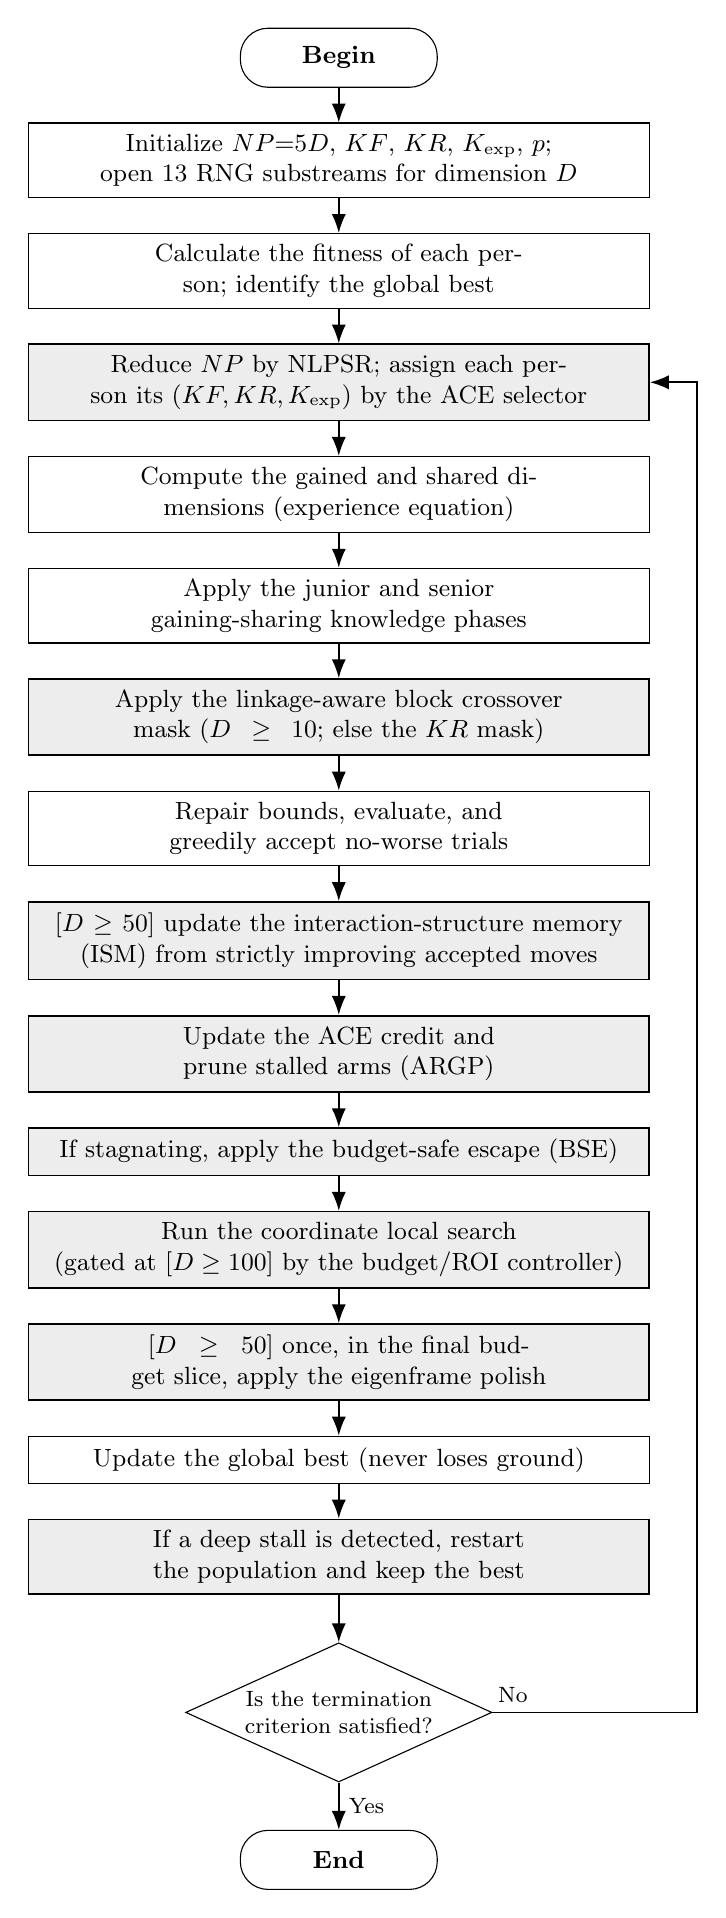
\begin{tikzpicture}[
  font=\small,
  node distance=4.4mm,
  term/.style={rectangle, rounded corners=10pt, draw=black, fill=white,
               minimum width=2.5cm, minimum height=0.75cm, align=center},
  proc/.style={rectangle, draw=black, fill=white, text width=7.6cm,
               minimum height=0.6cm, align=center, inner sep=4pt},
  new/.style={rectangle, draw=black, line width=0.6pt, fill=black!7,
              text width=7.6cm, minimum height=0.6cm, align=center, inner sep=4pt},
  dec/.style={diamond, aspect=2.2, draw=black, fill=white, align=center,
              inner sep=1pt, text width=2.5cm, font=\footnotesize},
  arr/.style={-{Latex[length=2.4mm]}, semithick},
  lbl/.style={font=\footnotesize},
]
\node (begin) [term] {\textbf{Begin}};
\node (init)  [proc, below=of begin]
  {Initialize $NP{=}5D$, $KF$, $KR$, $K_{\exp}$, $p$; open 13 RNG substreams for
   dimension $D$};
\node (fit)   [proc, below=of init]
  {Calculate the fitness of each person; identify the global best};
\node (adapt) [new, below=of fit]
  {Reduce $NP$ by NLPSR; assign each person its $(KF,KR,K_{\exp})$ by the
   ACE selector};
\node (dims)  [proc, below=of adapt]
  {Compute the gained and shared dimensions (experience equation)};
\node (phase) [proc, below=of dims]
  {Apply the junior and senior gaining-sharing knowledge phases};
\node (cross) [new, below=of phase]
  {Apply the linkage-aware block crossover mask ($D\ge10$; else the $KR$ mask)};
\node (acc)   [proc, below=of cross]
  {Repair bounds, evaluate, and greedily accept no-worse trials};
\node (sgsm)  [new, below=of acc]
  {$[D\ge50]$ update the interaction-structure memory (ISM) from strictly
   improving accepted moves};
\node (argp)  [new, below=of sgsm]
  {Update the ACE credit and prune stalled arms (ARGP)};
\node (bse)   [new, below=of argp]
  {If stagnating, apply the budget-safe escape (BSE)};
\node (sub)   [new, below=of bse]
  {Run the coordinate local search
   \mbox{(gated at $[D\ge100]$ by the budget/ROI controller)}};
\node (pol)   [new, below=of sub]
  {$[D\ge50]$ once, in the final budget slice, apply the eigenframe polish};
\node (gbest) [proc, below=of pol]
  {Update the global best (never loses ground)};
\node (rst)   [new, below=of gbest]
  {If a deep stall is detected, restart the population and keep the best};
\node (dec)   [dec, below=6mm of rst] {Is the termination criterion satisfied?};
\node (end)   [term, below=6mm of dec] {\textbf{End}};
% edges (single vertical spine)
\foreach \a/\b in {begin/init,init/fit,fit/adapt,adapt/dims,dims/phase,
                   phase/cross,cross/acc,acc/sgsm,sgsm/argp,argp/bse,bse/sub,sub/pol,
                   pol/gbest,gbest/rst,rst/dec}
  \draw [arr] (\a) -- (\b);
\draw [arr] (dec) -- node[lbl,right]{Yes} (end);
% loop-back (No) on the right, up to the NLPSR/ACE step
\coordinate (rail) at ($(dec.east)+(2.6cm,0)$);
\draw [arr] (dec.east) -- node[lbl,above,pos=0.1]{No} (rail)
      -- (rail |- adapt.east) -- (adapt.east);
\end{tikzpicture}
\end{document}
